% 2. Fragen zur Vorbereitung

\chapter{Theoretischer Hintergrund}
\label{chap:fvz}

\section{Arten und Vergleich der Mikroskope}
\label{sec:artenEM}

\subsection*{Raster-Elektronenmikroskop (REM)}
Bei einem REM wird durch einen Elektronenstrahl die zu untersuchende Probe zeilenförmig abgerastert. Dabei wird die Topografie (Oberfläche), die Kristallstruktur un Materialunterschiede der Probe auf einen Bildschirm mittels Sekundärelektronen (SE, inelastische Stöße) und Rückstoßelektronen (RE, elastische Stöße) mit entsprechenden Detektoren abgebildet. Weiterhin lässt ein REM eine Röntgenanalyse zu, wodurch auch eine Elementanalyse der Probe möglich ist. \citep{RasterEM}
\begin{itemize}
    \item Auflösung: $\sim$ \SI{10}{\nano\metre}\\
    Das Auflösungvermögen ist dabei von dem Strahlendurchmesser und dem Abbildungsignal abhängig und beträgt zwischen \SI{1}{\nano\metre} $\sim$ \SI{2}{\nano\metre} in günstigen Verhältnissen. \citep{WikiREM}
    \item Eindringtiefe: $\sim$ \SI{1}{\micro\metre}
    \item Probe: Vakuumstabil und trocken mit leitender Oberflächenschicht 
\end{itemize}
Das REM und seine Funktionsweise wird in weiteren Kapitel noch genauer betrachtet.

\subsection*{Transmission-Elektronenmikroskop (TEM)}
Bei einem TEM werden dünne Probe wird mit Elektronen durchstrahlt, welche durch die Streuung ihre Bewegungsrichtung ändern und ihre Energie durch inelastische Stöße verlieren. Die Elektronen, welche das Material durch elastische Stöße unter Erhaltung des Eintrittswinkels verlassen, werden in der hinteren Brennebene fokussiert. Die gestreuten Elektronen werden mit einer Blende abgeschirmt. Entweder wird dann das \textit{Zwischenbild} (vergrößertes Lichtbild) oder das \textit{Elektronenbeugungsbild} (Fokusebene) betrachtet. 
\begin{itemize}
    \item Auflösung: einige \si{\nano\metre} bis \si{\micro\metre}\\
    Dabei hängt die Auflösung von der Beschleuigungsspannung (80 $\sim$ 400\si{\kilo\volt}) und der Materialdicke ab. 
    \item Probe: Ultradünne Schnitte notwendig (10–\SI{100}{\nano\metre}) \citep{WikiTEM}
\end{itemize}
\newpage
\subsection*{Lichtmikroskop (LM)}
Beim LM werden stark vergrößerte Bilder von kleinen Strukturen oder Objekten mit Hilfe von Licht und optischen System aus Linsen erzeugt.
\begin{itemize}
    \item Auflösung: \SI{0,2}{\micro\metre} $\sim$ \SI{0,3}{\micro\metre}\\
    Wird durch die physikalischen Gesetzmäßigkeiten bestimmt und hängt somit von der Wellenlänge ab. 
    \item Probe: Für gut erkennbare Strukturen im Bild muss die Probe ausreichend Kontrast enthalten. \citep{WikiLM}
\end{itemize}

\subsection*{(REM,TEM) vs LM}
\begin{itemize}
    \item[\textcolor{green}{\textbf{+}}] Licht mit viel größerer Wellenlänge (\SI{380}{\nano\metre}) als Elektronen (Welle-Teilchen-Dualismus)(\SI{5}{\nano\metre}) $\Rightarrow$ Erheblich bessere Auflösung
    \item[\textcolor{red}{\textbf{-}}] (REM,TEM) benötigt Vakuum im Gang des Elektronenstrahl imd elktromagnetische Linsen, während eine LM \enquote{nur} Glaslinsen benötigt $\Rightarrow$ Höherer technischer Aufwand \citep{RuppelEM}
\end{itemize}

\subsection*{REM vs TEM}
\begin{itemize}
    \item[\textcolor{green}{\textbf{+}}] Probenpräpartion einfacher, da keine ultradünnen Schnitte der Probe erzeugt werden müssen
    \item[\textcolor{green}{\textbf{+}}] 3D-Abbildung der Oberfläche des Objekts $\Rightarrow$ leicht verständliche Bilder 
    \item[\textcolor{red}{\textbf{-}}] geringere Vergrößerung und Auflösung
    \item[\textcolor{red}{\textbf{-}}] Keine Aussage über innere Struktur der Probe \citep{RuppelEM} 
\end{itemize}

\section{Aufbau eines Raster-Elektronenmikroskops}
\label{sec:aufbau}
In einer Mikroskopsäule wird der Durchmesser des Elektronenstrahls durch die Kondensorlinsen und der Aparturblende (\SI{50}{\milli\metre}) elektronenoptisch verkleinert. Der Elektronenstrahl selbst entsteht durch eine thermische Wolframkathode erzeugte Elektronenwolke, welche durch die Anode nach unten beschleunigt und durch die Stigmatoren fokussiert wird. Ablenkspulen sorgen dann  für zeilenförmigen Abrasterung der Probe durch den Elektronenstrahl. \citep{RasterEM} Aufbau ist in Abbildung \ref{image:aufbau} dargestellt. Die verschiedenen Elektronen werden dann von einem Everheart-Thornley-Detektor und Halbleiterdetektor registriert und die entstehende Röngtenstrahlung von einem EDX-Detektor. Dabei dienen die registrierten Elektronen als Signal zur Helligkeitsmodulation des Bildes. \citep{RasterEM}
\begin{center}
    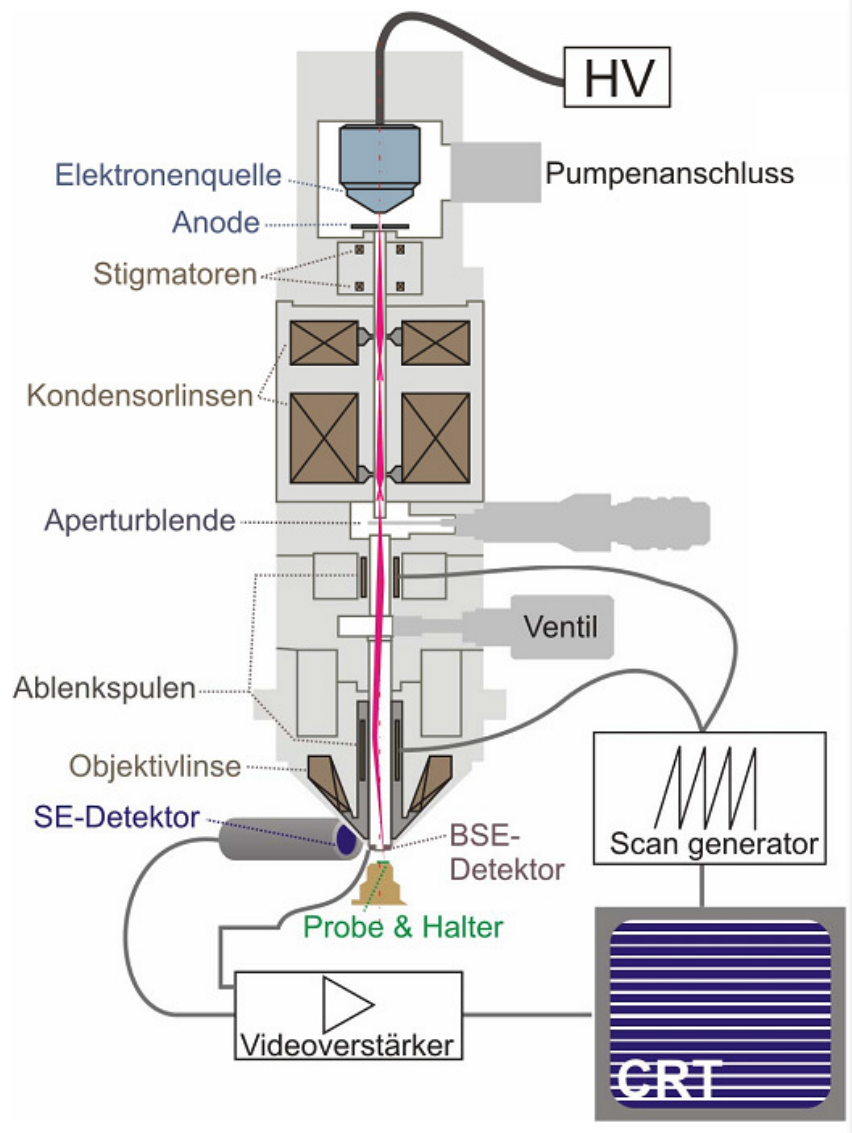
\includegraphics[scale=0.25]{AufbauREM.png}
    \captionof{figure}{Aufbau Raster-Elektronenmikroskop}
    \label{image:aufbau}
\end{center}

\section{Wechselwirkung der Elektronen mit Materie}
\label{sec:elektrons}
Durch Wechselwirkung des Primärelektronenstrahls (PE) mit der Materie entstehen unterschiedliche Signale, welche in Abbildung \ref{image:signal} dargestellt sind.
\begin{center}
    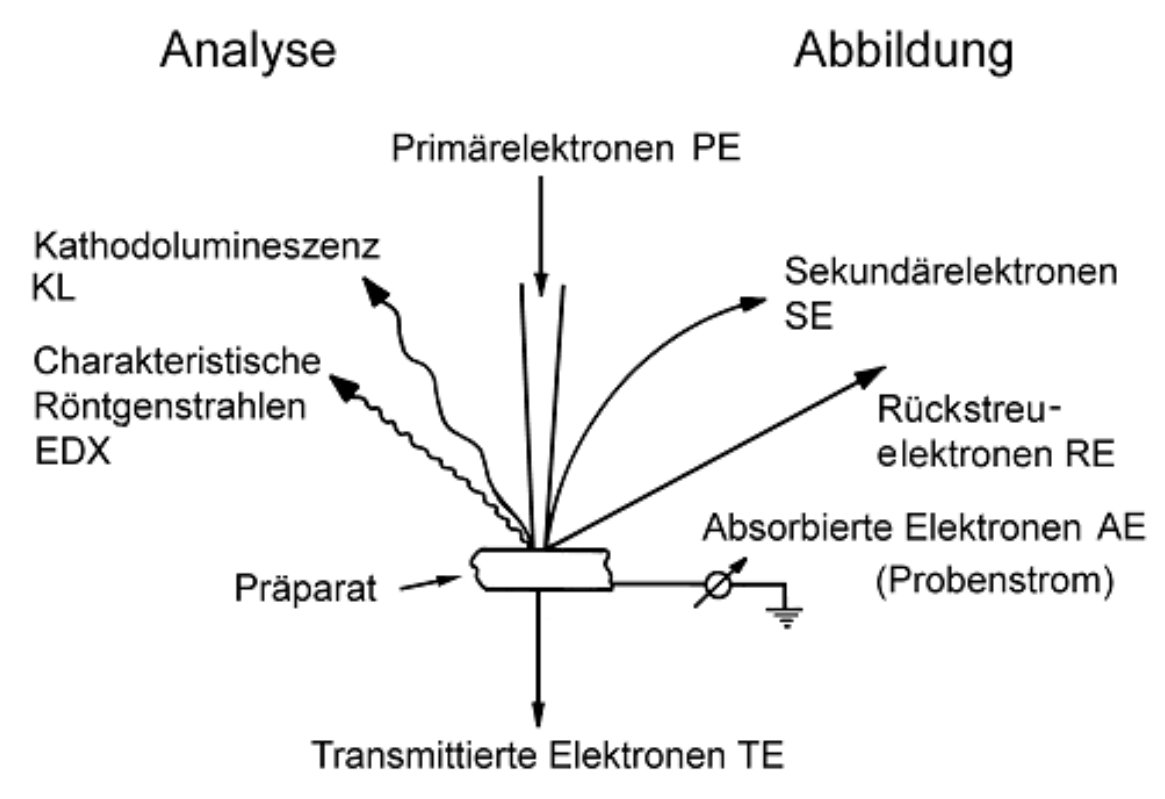
\includegraphics[scale=0.25]{Signalentstehung.png}
    \captionof{figure}{Signale eines REMs}
    \label{image:signal}
\end{center}
Das Volumen, in dem die Elektronen des Primärelektronenstrahls wechselwirken, heißt Streubirne oder Elektronendiffusionswolke, wobei die Reichweite vom gewählten Probenmaterial und der Anregungsspannung abhängt. 
\begin{center}
    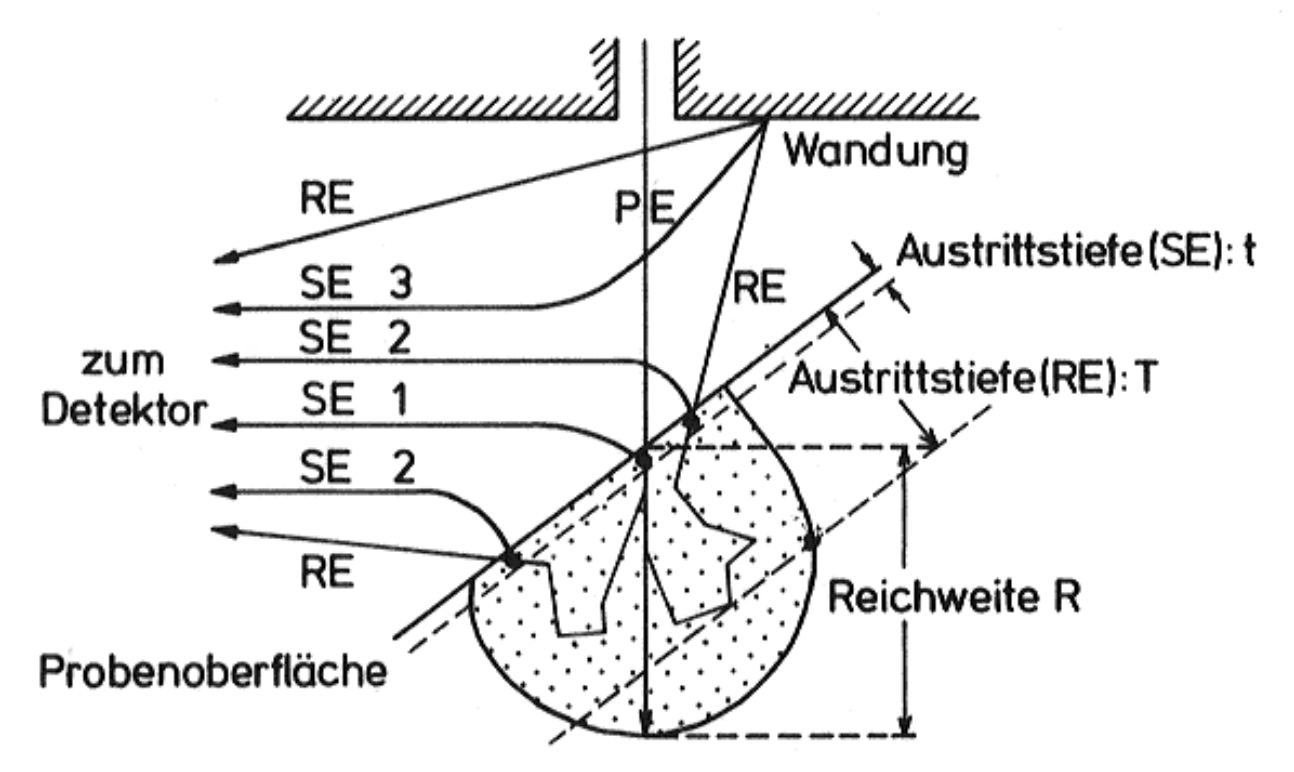
\includegraphics[scale=0.2]{Elektronendiffusionswolke.png}
    \captionof{figure}{Elektronendiffusionswolke}
    \label{image:wolke}
\end{center}
Durch Eindringen des PE entstehen durch unelastische Streuung langsame \textbf{\textit{Sekundärelektronen (SE)}} mit Energie < \SI{50}{\electronvolt} mit wahrscheinlichster Energie $\left\langle E\right\rangle=\SI{2,5}{\electronvolt}$, welche aus der $t =$ 1-\SI{10}{\nano\metre} stammen und zur Hochauflösung des REM führen. \citep{RasterEM} Somit tragen SE maßgeblich zu den dem sogenannten \textit{Topografiekontrast} bei. \citep{WikipolyREM} Elektronen, welche elastisch an Atomkerne gestreut werden und diesen unter großen Winkel verlassen, werden als \textbf{\textit{Rückstoßelektronen (RE)}}. REs haben dabei eine Energie > \SI{50}{\electronvolt}, worunter auch schnellere SE fallen, aber diese sind von REs nicht unterscheidbar sind. Dabei stammen die ausgelösten REs aus einer Materialtiefe $T=$0,1-\SI{1}{\micro\metre} und sind somit verantwortlich für den \textit{Materialkontrast}. Auch hängt die Ausbeute der REs von der Kernladungszahl des Materials ab. \citep{RasterEM} \citep{WikipolyREM} Die REs können auch beim Austreten weitere SEs erzeugen, was man gut Anhand des \textit{Kantenkontrast} erkennen kann. \citep{RasterEM} 

SE werden dann in Gruppen unterteilt:
\begin{itemize}
    \item[(SE1)] Aus PE im Materail erzeugte SEs
    \item[(SE2)] Aus RE im Material erzeugte SEs 
    \item[(SE3)] Aus RE außerhalb des Materials erzeugte SEs   
\end{itemize}

Bis zu einer Reichweite von $R=\SI{500}{\nano\metre}$ entsteht eine Wechselwirkung des PE-Strahls mit der Probe, wobei Elektronen aus der Atomhülle geschlagen werden. Dabei fallen Elektronen aus höheren Zuständen nach und es entsteht dabei Röntgenstrahlung, wobei diese Strahlung charakteristisch für das jeweilige Element ist. Die emittierende Strahlung kann dann noch ein Elektron aus einer höheren Schale herausschlagen, was als Auger-Elektron registriert wird. Bei Kernen mit kleiner Ordnungszahl ($Z$<20) dominiert die Emission von Auger-Elektronen, bei
höheren Ordnungszahlen überwiegt die Emission von charakteristischer Röntgenstrahlung.

\section{Detektoren}
\label{sec:detect}

\section{Abbildungsfehler und Kontraste}
\label{sec:imageErrorKontrast}

\section{Röntgenanalyse}
\label{sec:roentgen}
